\chapter{Billedkomprimering med diskret cosinustransformation} \label{chapter:DCT}
I dette kapitel udarbejde en billedkomprimeringsalgoritme med tab med udgangspunkt i den
en diskret cosinustransformation. Før denne forklares, er det nødvendigt at undersøge
den diskrete Fouriertransformation, som den stammer fra.
\section{Diskret Fouriertransformation}
Inden for signalbehandling er den Diskrete Fouriertransformation (DFT) et kendt værktøj. Transformationen er en lineær transformation, som udtrykker et signal på bølgeform ved sinus- og cosinusfunktioner [\citet{thefouriertransform}, afsnit 1]. De fleste signaler er på bølgeform og kan derfor beskrives ved sinus- og cosinusfunktioner gennem DFT.\\
Signalerne kan beskrives i to domæner
\begin{itemize}
\item \textit{Tidsdomænet}\\
		Signalet beskrives ved funktionsværdier til tiden $t$, $f(t)$.
\item \textit{Frekvensdomænet}\\
		Signalet beskrives ved amplitude og fase for en frekvensfunktion.
\end{itemize}
Regneoperationer i tidsdomænet har tilsvarende regneoperationer i frekvensdomænet, som ofte er beregningsmæssigt simplere [\citet{nbtwiki}, afsnit 2]. Af denne grund bruges den diskrete Fouriertransformation til signalbehandling.\\
Transformationen har desuden den egenskab, at den energikomprimerer signalet, som behandles. Energikomprimering betegner en transformations evne til at udtrykke mange signalværdier med høje korrelationer i domænet som færre koefficienter med lav korrelation i kodomænet [\citet{smcnus_energy}, s. 1]. Koefficienterne i frekvensdomænet fortæller i hvor høj grad de enkelte basisfunktioner er repræsenteret i tidsdomænet - høje koefficienter viser en høj optræden af den tilhørende basisfunktion, mens lave koefficienter viser en lav optræden af den tilhørende basisfunktion.

Når DFT udtrykker korrelerede signalværdier som ukorrelerede koefficienter i frekvensdomænet, betyder det også, at transformationen ikke formår at lave energikomprimering i høj grad, hvis signalværdierne er ukorrelerede. Dette betyder at, hvis der ønskes høj energikomprimering, skal DFT kun bruges på signaler, som består af korrelerede værdier.

I billedkomprimering er det, som tidligere beskrevet, interessant at udtrykke et billede ved færre værdier, da der derfor er færre værdier at gemme. DFT kan være et værktøj til dette. Et billede  består netop af korrelerede værdier og DFT kan derfor bruges.

Det viser sig imidlertid, at der findes et bedre værktøj til transformation af korrelerede signalværdier til ukorrelerede koefficienter. Transformationen kaldes den diskrete cosinustransformation (DCT), og er udledt fra DFT [\citet{dft_argument}, s. 3]. Udledningen ses i appendiks \vref{DCT_udledning}.\\
DCT udmærker sig inden for billedbehandling på flere områder i forhold til DFT:
\begin{enumerate}
\item \textit{Energikomprimering}\\
	DCT opnår højere energikomprimering end DFT [\citet{smcnus_energy}, s. 3 og 5]. Den formår at udtrykke informationer om signalværdier i tidsdomænet som færre koefficienter i frekvensdomænet end DFT formår. Det er ønskværdigt at udtrykke mange informationer ved få koefficienter i billedkomprimering.
\item \textit{Reelle tal}\\
	DCT benytter sig udelukkende af reelle tal i de transformerede koefficienter, hvorimod DFT benytter sig af både reelle og komplekse tal som koefficienter. Det er ønskværdigt, at regne udelukkende med reelle tal, da dette forsimpler den videre behandling af signalet.
\end{enumerate}
Der findes desuden en transformation, som bygger på sinusfunktioner - den diskrete sinustransformation (DST). Denne transformerer også signalværdier om til frekvenskoefficienter, men energikomprimerer ikke godt - den er ringere end både DFT og DCT [\citet{smcnus_energy}, s. 5].

Som følge af ovenstående grunde er der valgt at bruge DCT i den mest udbredte open-source komprimeringsstandard; JPEG.\\
På baggrund af at DCT
\begin{itemize}
\item[-] har bedre energikomprimering end DFT [\citet{smcnus_energy}, s. 5], og dermed skal færre koefficienter end DFT bruges til at danne en god approksimation af et signal [\citet{dft_argument}, s. 5]
\item[-] ofte bruges i billedbehandling [\citet{DTT}, s. 1]
\item[-] bruges i JPEG [\citet{dft_argument}, s. 1]
\end{itemize}
tages der i denne opgave udgangspunkt i DCT til at udføre billedkomprimeringer.
\subsection{JPEG}
Joint Photographic Experts Group udgav i 1992 den første JPEG-standard, som komprimerede og dekomprimerede billeder efter en bestemt algoritme. Et program, som kan gøre dette, kaldes en codec. Standarden er open source, og er siden 1992 blevet forbedret flere gange. I denne rapport undersøges en simpel og tidlig version.\\
JPEG gør brug af fire skridt i sin algoritme for at komprimere et billede fra dets fulde størrelse til en fil af mindre størrelse. Den inverse algoritme bruges til at dekomprimere en JPEG-fil til et billede. Da JPEG er en ikke-tabsfri komprimeringsalgoritme, er det dekomprimerede billede kun en efterligning af det originale. [\citet{whydomath_basic}, afsnit 1-7].\\
De fire skridt, som forklares nærmere i et senere afsnit, ser ud som følgende
\begin{enumerate}
\item \textit{Forbehandling af billede}\\
	Forbehandlingen indebærer at dele billedet op i kvadratiske undermatricer af 64 pixels. Dette gøres for at gøre den videre behandling af billedet med den diskrete cosinustransformation mere effektiv. Derudover trækkes 128 fra hver indgang i hver undermatrix for at centrere undermatricerne omkring nul.
\item \textit{Diskret cosinustransformation}\\
	Den diskrete cosinustransformation energikomprimerer billedet ved at udtrykke korrelerede signalværdier som dekorrelerede koefficienter i frekvensdomænet.
\item \textit{Kvantisering}\\
	Kvantiseringen fjerner mindre vigtige informationer om billedet ved at fjerne de dekorrelerede koefficienter, som ikke er vigtige i forhold til de korrelerede signalværdier. Dette skridt gør algoritmen ikke-tabsfri.
\item \textit{Entropikodning}\\
	Entropikodningen opstiller en statistisk model over de kvantiserede koefficienter og koder dem i strenge bestående af 0 og 1, som kan gemmes effektivt i en fil, som er mindre end den oprindelige billedfil.
\end{enumerate}
For at forstå hvorfor og hvordan algoritmen virker er det nødvendigt først at forstå den diskrete cosinustransformation. Derfor bliver dette skridt forklaret først.
\subsection{Diskret Cosinustransformation}\label{sec:DCT}
En diskret cosinustransformation er en lineær transformation, som afbilder en $n$-dimensionel vektor fra domænet $\mathbb{R}^n$ til kodomænet $\mathbb{R}^n$ - altså har transformationen samme kodomæne som domæne. Basisvektorerne i transformationen udledes fra cosinusfunktioner med forskellige frekvenser. Som følge af dette bliver den $n$-dimensionelle vektor afbildet ind i frekvensdomænet - den udtrykkes som en sum af cosinusfunktioner med forskellige frekvenser. Et eksempel på en funktion udtrykt ved bølgefunktioner ses i figur \vref{fig:frequencydomain}.

Som tidligere nævnt er den diskrete cosinustransformation udledt fra den diskrete Fouriertransformation. Udledningen ses i appendiks \vref{DCT_udledning}.

DCT bruges i udstrakt grad i signalbehandling på grund af dens høje energikomprimering. DCT kan altså komprimere meget signalværdi ned til få værdier i frekvensdomænet og dermed udtrykke signalværdier med stor korrelation som koeffiencienter med lav eller ingen korrelation [\citet{lokminglui_DCT}, s. 1]. Transformationen fungerer dog bedst, når signalværdierne som transformeres, har en vis korrelation - hvis dette ikke er tilfældet, vil der ikke blive opnået gode resultater med transformationen.

DCT er imidlertid ikke den eneste transformation, som kan dekorrelere signalværdier. En anden kendt transformation er Karhunen-Loève transformationen. Denne transformation transformerer som cosinustransformationen også korrelerede koefficienter til dekorrelerede koefficienter. Karhunen-Loeve udmærker sig ved at tilpasse sig hvordan signalet ser ud, for således at kunne energikomprimere meget effektivt - transformationen afhænger altså af signalet. Dette gør transformationen i stand til at lave den mest effektive energikomprimering [\citet{lokminglui_DCT}, s. 15]. Det er imidlertid ikke tidsmæssigt effektivt at komponere en ny transformation, hver gang et nyt signal behandles og derfor bruges den diskrete cosinustransformation i JPEG. Denne har en algoritme, som genererer en generel transformation, der kan bruges på mange datasæt [\citet{electronic_engineering}, s. 2].

Da DCT er en lineær transformation, kan den bruges i billedbehandling til at energikomprimere digitale billeder, som har stor korrelation mellem nærliggende pixels.\\
\begin{figure}[htbp]
\centering
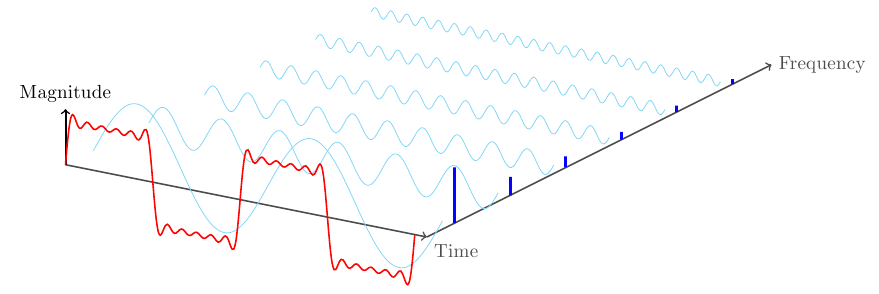
\includegraphics[width=0.7\textwidth]{Billeder/frequencydomain.png}
\caption{Signal (rød) og cosinusbølger (blå kurver) samt amplituden (søjler)[\citet{frequency_image}, \textit{Update 1}].}
\label{fig:frequencydomain}
\end{figure}
Den diskrete cosinustransformation, som kan udledes fra den diskrete Fouriertransformation, kan transformere i både én og to dimensioner. I denne opgave benyttes den todimensionelle. I ligning \vref{eq:DCTeq} ses den todimensionelle $n$-punkt diskrete cosinustransformation, hvor $T:\mathbb{R}^n \longrightarrow \mathbb{R}^n$ transformerer til en matrix indeholdende dekorrelerede koeffecienter. Matricen der transformeres, vil fremover refereres til som $A$. 
\begin{equation}
T_{(i,\ j)}=\sum\limits_{x=0}^{n-1} \sum\limits_{y=0}^{n-1} f(x,\ y) \cdot \alpha(i) \cdot \alpha(j) \cdot \cos\left(\frac{(2x+1) \cdot i \cdot \pi}{2n}\right) \cdot \cos\left(\frac{(2y+1) \cdot j \cdot \pi}{2n}\right)
\label{eq:DCTeq}
\end{equation} [\citet{guillermo_sapiro}, 7:12-11:10]\\
Hvor
\begin{itemize}
\item $T_{(i,\ j)}:$ indgang $(i,\ j)$ i den transformerede matrix ved DCT
\item $f(x,\ y):$ indgang $(x,\ y)$ i A
\item $n:$ matricens dimension
\item $\alpha(i)=\alpha(j)= \begin{cases}
					\sqrt{\frac{1}{n}} \ hvis \ i = 0\\
					\sqrt{\frac{2}{n}} \ hvis \ i \neq 0
					\end{cases}$
\end{itemize}
Det er værd at bemærke, at indgangene i matricen går fra $(0,\ 0)$ til $(n-1,\ n-1)$ i en $n \times n$ matrix. Ydermere er $\alpha(i)$  og $\alpha(j)$ normaliseringsfaktorer [\citet{normalization}, s. 96].

Ligning \ref{eq:DCTeq} bruges i denne opgave ikke til at beregne de transformerede koefficienter, da det beregningsmæssigt ikke er effektivt. Til dette bruges i stedet cosinustransformationen på matrixform, hvilket uddybes senere i dette afsnit. Ligning \ref{eq:DCTeq} er imidlertid god til at illustrere princippet bag transformationen, da det er tydeligt, hvordan cosinusfunktioner indgår i transformationen. Dette undersøges nu.

Det ses af ligning \vref{eq:DCTeq}, at hver transformeret indgang er summen af produktet af de 64 indgange i $A$ og en koefficient fra en cosinusfunktion. For hver række $f(x,\ y)$ holdes $x$ konstant gennem de otte søjler, hvor $y$ går fra $0-7$. Dette giver koefficienter, der alle ligger på en cosinuskurve. Hver gang en ny række $x$ påbegyndes, ændres amplituden af cosinusbølgen, som koefficienterne ligger på. Når en ny transformeret indgang $T_{(i,\ j)}$ beregnes, ændres $i$ og/eller $j$, og frekvensen af cosinusfunktionerne i transformen bliver højere. Altså bliver hver transformeret indgang et unikt aftryk af forskelligt svingene cosinusfunktioner og værdierne i matricen til billedet $A$.

For at illustrere princippet bag de skiftende amplituder og frekvenser af cosinusbølgerne som koefficienterne ligger på, er et sæt af to grafer for cosinustransformationen illustreret i figurerne \ref{fig:frekeksu1v1} og \ref{fig:frekeksu1v2}. Disse er tegnet ved brug af transformationen i ligning \vref{eq:DCTeq} for henholdsvis $T(1,\ 1)$ og $T(1,\ 2)$ og for $n=8$. For hver af funktionerne fremkommer otte bølger, og på hver af disse ligger de otte koefficienter ligeligt fordelt. På figur \ref{fig:cosko} ses de otte punkter på én af bølgerne for $T(0,\ 0)$ [\citet{whydomath_dct}, afsnit 3].

\begin{figure}[!h]
\begin{minipage}[b]{0.5\linewidth}
\centering
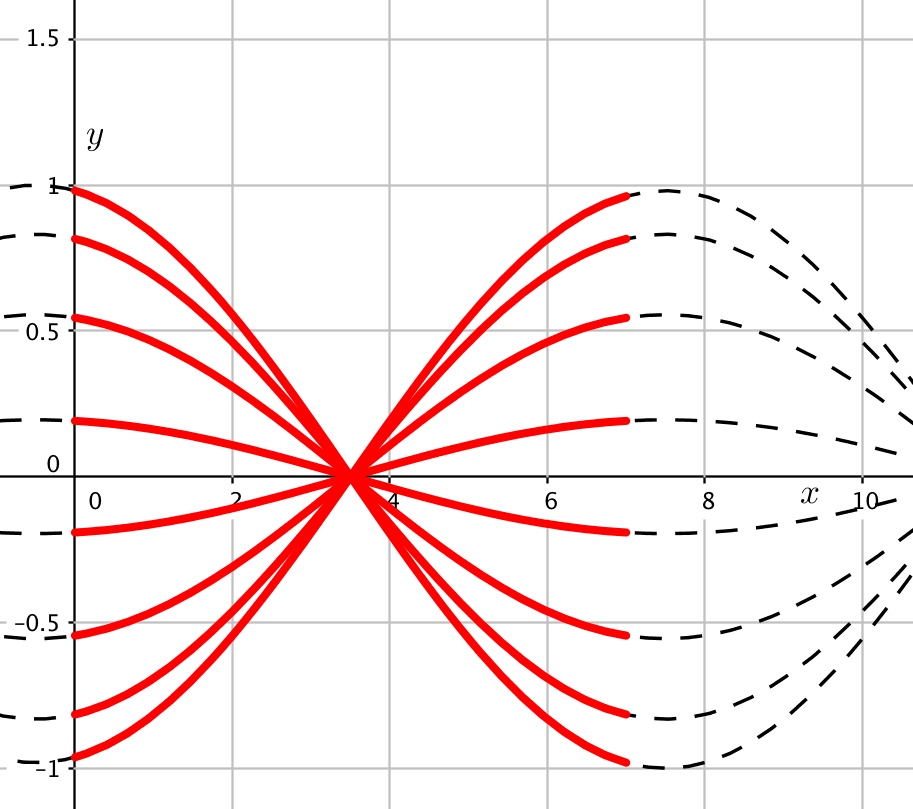
\includegraphics[width=0.6\textwidth]{Billeder/Frekvens-eksempelu1v1.png}
\caption{Bølger for hver række for $T(1,\ 1)$.} %tegnet ved brug af ligning \vref{eq:DCTeq}. På hver af disse bølger ligger 8 ligeligt fordelte koefficienter, som multipliceres med signalværdierne.}
\label{fig:frekeksu1v1}
\end{minipage}
\begin{minipage}[b]{0.5\linewidth}
\centering
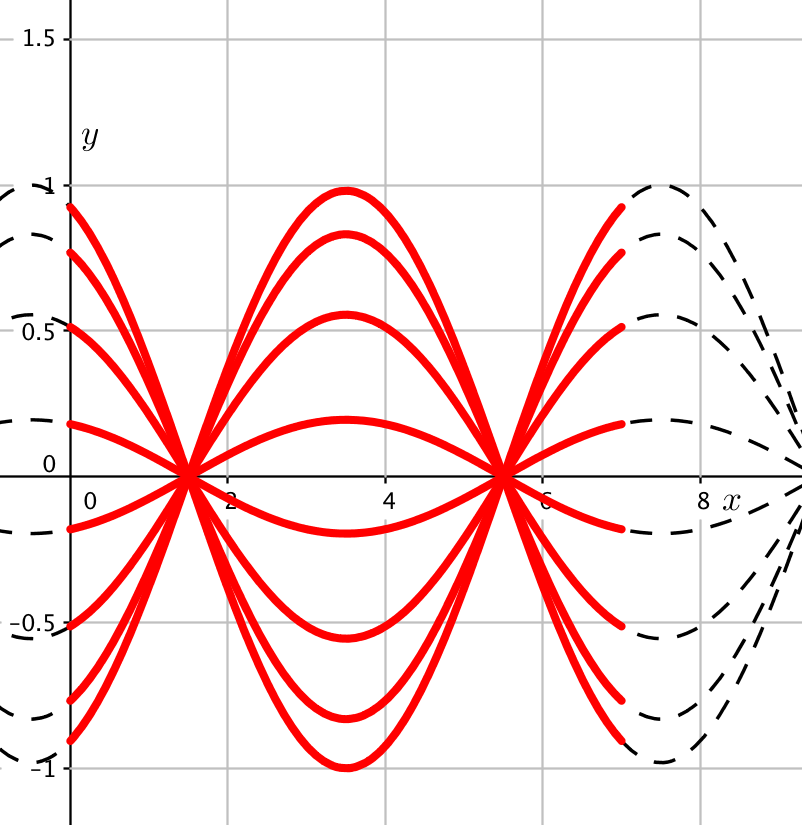
\includegraphics[width=0.5\textwidth]{Billeder/Frekvens-eksempelu1v2.png}
\caption{Bølger for hver række for $T(1,\ 2)$.}
\label{fig:frekeksu1v2}
\end{minipage}
\end{figure}

\begin{figure}[htbp]
\centering
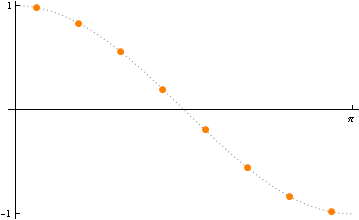
\includegraphics[width=0.4\textwidth]{Billeder/coskoefficienter.png}
\caption{Koefficienterne for $T(1,\ 1)$ og $f(0,\ y)$ afmærket som punkter på en cosinusbølge.}
\label{fig:cosko}
\end{figure}

Det ses desuden på figur \vref{fig:cosko}, at koefficienterne tilsammen har sum lig nul. Der er altså lige mange positive og negative koefficienter i alle bølgerne med undtagelse af den første, som udelukkende består af koefficienten $\frac{\sqrt{2}}{2}$.\\
At hele den første række kun indeholder positive indgange bidrager til energikomprimeringen. Hvis A indeholder lignende værdier, vil indgang $(0,\phantom{i}0)$ have stor numerisk værdi efter transformationen. Derfor kan en stor del af informationerne koncentreres i denne ene indgang. På samme måde vil resultatet af at prikke en vektor med ens indgange, $\vec{v}= \begin{bmatrix} v_1 & v_1 & \hdots & v_1 \end{bmatrix}$ med en hvilken som helst samling af koefficenter fra en cosinusbølge beregnet ved $i=0,\ldots,7$ blive lig nul. Resultatet af at prikke en vektor, med indgange der næsten er ens med koefficienterne, vil blive tæt på eller lig nul [\citet{whydomath_dct}, afsnit 4]

Koefficienten i indgang $(0,\phantom{i}0)$ omtales som DC koefficienten eller Direct Current. De resterende 63 koefficienter kaldes for AC koefficienter eller Alternating Current. Navnene stammer fra transformationens historiske brug i analyse af elektriske kredsløb og refererer til basisfunktionerne i transformationen, som for DC koefficienten er konstant som jævnstrøm, men de oscillerer som vekselstrøm for de resterende koefficienter [\citet{lokminglui_DCT}, s. 5].

De transformerede koefficienter udtrykker bestemte mønstre i signalet. Mønstrene for hver koefficient ses i figur \vref{fig:frekvens_matrix}, hvor bølgetoppene og -dalene i cosinusfunktionerne (og dermed negative og positive koefficienter) er henholdsvis sorte og hvide. Denne figur illustrerer hvordan transformationen behandler forskellige slags mønstre i signalet - mønstre som ligner signalet vil have høje koefficienter. Bemærk at DC koefficienten er en koefficient for et ensfarvet mønster eller signal.
\begin{figure}[htbp]
\centering
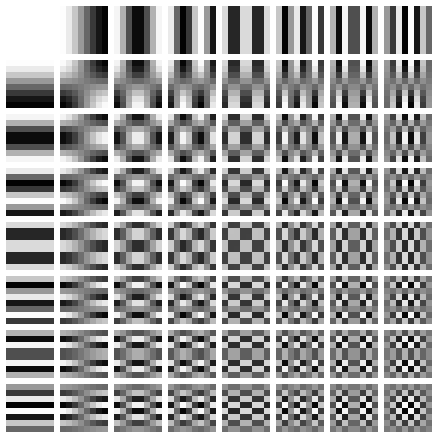
\includegraphics[width=0.35\textwidth]{billeder/frekvensmatrix.png}
\caption{Repræsentation af de 64 forskellige basisfunktioner i cosinustransformationen af længde $n = 8$. Mønstrene hører til koefficienterne, som fås ved transformation af et signal. Koefficienternes størrelse fortæller hvor meget, det tilhørende mønster optræder i signalet.}
\label{fig:frekvens_matrix}
\end{figure}
Indgangene i den transformerede matrix er koefficienterne, hvorved disse mønstre er repræsenteret i signalet. Altså kan signalet genskabes ved en lineær kombination af disse mønstre.

I dette projekt udføres beregninger og dermed også transformationen i Python. Til dette er det beregningsmæssigt nemmere og hurtigere at regne med DCT på matrixform.

I udledningen af DCT i appendiks \vref{DCT_udledning} ses formlen for den todimensionelle DCT, hvor ligning \vref{eq:soejlevektor} viser, hvordan hver enkelt søjle i en matrix for en n-punkts DCT beregnes. Da der i denne opgave regnes med matricer af størrelsen $8 \times 8$, vises der i ligning \ref{eq:DCTmatrix} en matrix beregnet ved $n=8$ - altså en $8 \times 8$-matrix.
%\begin{align}
%	y_{(i,j)} = C(i) \sqrt{\frac{2}{n}} \cos\left(\frac{(2 \cdot j-1) \cdot (i-1)\pi}{2n}\right)
%\label{eq:DCTmatrixform}
%\end{align}
%Hvor
%\begin{itemize}
%		\item{$C(i)= \begin{cases}
%			\frac{1}{\sqrt{2}} \ hvis \ i = 1\\
%			1\ \ \ hvis \ i \neq 1
%		\end{cases}
%		$}
%		\item{$y_{(i,j)}=$ indgang $(i,j)$}
%		\item{$n =$ matricens dimensioner n$\times$n}
%\end{itemize}
%Matricen beregnet ved formel \vref{eq:DCTmatrixform} hvor $n=8$ ses i ligning \ref{eq:DCTmatrix}.
\begin{equation}
U=\frac{1}{2}
\begin{bsmallmatrix}
	\frac{\sqrt{2}}{2}	& \frac{\sqrt{2}}{2}		& \frac{\sqrt{2}}{2}		& \frac{\sqrt{2}}{2}		& \frac{\sqrt{2}}{2}		& \frac{\sqrt{2}}{2}		& \frac{\sqrt{2}}{2}		& \frac{\sqrt{2}}{2}		\\
	\cos(\frac{\pi}{16})		& \cos(\frac{3\pi}{16})	& \cos(\frac{5\pi}{16})	& \cos(\frac{7\pi}{16})	& \cos(\frac{9\pi}{16})	& \cos(\frac{11\pi}{16})	& \cos(\frac{13\pi}{16})	& \cos(\frac{15\pi}{16})		\\
	\cos(\frac{2\pi}{16})	& \cos(\frac{6\pi}{16})	& \cos(\frac{10\pi}{16})	& \cos(\frac{14\pi}{16})	& \cos(\frac{18\pi}{16})	& \cos(\frac{22\pi}{16})	& \cos(\frac{26\pi}{16})	& \cos(\frac{30\pi}{16})		\\
	\cos(\frac{3\pi}{16})	& \cos(\frac{9\pi}{16})	& \cos(\frac{15\pi}{16})	& \cos(\frac{21\pi}{16})	& \cos(\frac{27\pi}{16})	& \cos(\frac{33\pi}{16})	& \cos(\frac{39\pi}{16})	& \cos(\frac{45\pi}{16})		\\
	\cos(\frac{4\pi}{16})	& \cos(\frac{12\pi}{16})	& \cos(\frac{20\pi}{16})	& \cos(\frac{28\pi}{16})	& \cos(\frac{36\pi}{16})	& \cos(\frac{44\pi}{16})	& \cos(\frac{52\pi}{16})	& \cos(\frac{60\pi}{16})		\\
	\cos(\frac{5\pi}{16})	& \cos(\frac{15\pi}{16})	& \cos(\frac{25\pi}{16})	& \cos(\frac{35\pi}{16})	& \cos(\frac{45\pi}{16})	& \cos(\frac{55\pi}{16})	& \cos(\frac{65\pi}{16})	& \cos(\frac{75\pi}{16})		\\
	\cos(\frac{6\pi}{16})	& \cos(\frac{18\pi}{16})	& \cos(\frac{30\pi}{16})	& \cos(\frac{42\pi}{16})	& \cos(\frac{54\pi}{16})	& \cos(\frac{66\pi}{16})	& \cos(\frac{78\pi}{16})	& \cos(\frac{90\pi}{16})		\\
	\cos(\frac{7\pi}{16})	& \cos(\frac{21\pi}{16})	& \cos(\frac{35\pi}{16})	& \cos(\frac{49\pi}{16})	& \cos(\frac{63\pi}{16})	& \cos(\frac{77\pi}{16})	& \cos(\frac{91\pi}{16})	& \cos(\frac{105\pi}{16})	\\
\end{bsmallmatrix}
\label{eq:DCTmatrix}
\end{equation}
Magen til ligning \vref{eq:DCTeq} kan $U$ bruges til at opnå DCT transformationen, blot hvor en stor del af udregningerne er udført på forhånd. På matrixform prikkes $U$ med $A$, og derefter prikkes dette resultat med $U^T$. Transformationen ses i ligning \vref{eq:DCTtrans}. %I beregningerne bruges den transponerede matrix, som ses i ligning \Vref{eq:DCTmatrixT}.
%\begin{equation}
%U^T = \frac{1}{2}
%\begin{bmatrix}
%\frac{2}{\sqrt{2}} & \cos(\frac{\pi}{16}) & \cos(\frac{2 \cdot \pi}{16}) & \cos(\frac{3 \cdot \pi}{16}) & \cos(\frac{4 \cdot \pi}{16}) & \cos(\frac{5 \cdot \pi}{16}) & \cos(\frac{6 \cdot \pi}{16}) & \cos(\frac{7 \cdot \pi}{16}) \\
%\frac{2}{\sqrt{2}} & \cos(\frac{3 \cdot \pi}{16}) & \cos(\frac{6 \cdot \pi}{16}) & \cos(\frac{9 \cdot \pi}{16}) & \cos(\frac{12 \cdot \pi}{16}) & \cos(\frac{15 \cdot \pi}{16}) & \cos(\frac{18 \cdot \pi}{16}) & \cos(\frac{21 \cdot \pi}{16}) \\
%\frac{2}{\sqrt{2}} & \cos(\frac{5 \cdot \pi}{16}) & \cos(\frac{10 \cdot \pi}{16}) & \cos(\frac{15 \cdot \pi}{16}) & \cos(\frac{20 \cdot \pi}{16}) & \cos(\frac{25\cdot \pi}{16}) & \cos(\frac{30 \cdot \pi}{16}) & \cos(\frac{35 \cdot \pi}{16}) \\
%\frac{2}{\sqrt{2}} & \cos(\frac{7 \cdot \pi}{16}) & \cos(\frac{14 \cdot \pi}{16}) & \cos(\frac{21 \cdot \pi}{16}) & \cos(\frac{28 \cdot \pi}{16}) & \cos(\frac{35 \cdot \pi}{16}) & \cos(\frac{42 \cdot \pi}{16}) & \cos(\frac{49 \cdot \pi}{16}) \\
%\frac{2}{\sqrt{2}} & \cos(\frac{9 \cdot \pi}{16}) & \cos(\frac{18 \cdot \pi}{16}) & \cos(\frac{27 \cdot \pi}{16}) & \cos(\frac{36 \cdot \pi}{16}) & \cos(\frac{45 \cdot \pi}{16}) & \cos(\frac{54 \cdot \pi}{16}) & \cos(\frac{63 \cdot \pi}{16}) \\
%\frac{2}{\sqrt{2}} & \cos(\frac{11 \cdot \pi}{16}) & \cos(\frac{22 \cdot \pi}{16}) & \cos(\frac{33 \cdot \pi}{16}) & \cos(\frac{44 \cdot \pi}{16}) & \cos(\frac{55 \cdot \pi}{16}) & \cos(\frac{66 \cdot \pi}{16}) & \cos(\frac{77 \cdot \pi}{16}) \\
%\frac{2}{\sqrt{2}} & \cos(\frac{13 \cdot \pi}{16}) & \cos(\frac{26 \cdot \pi}{16}) & \cos(\frac{39 \cdot \pi}{16}) & \cos(\frac{52 \cdot \pi}{16}) & \cos(\frac{65 \cdot \pi}{16}) & \cos(\frac{78 \cdot \pi}{16}) & \cos(\frac{91 \cdot \pi}{16}) \\
%\frac{2}{\sqrt{2}} & \cos(\frac{15 \cdot \pi}{16}) & \cos(\frac{30 \cdot \pi}{16}) & \cos(\frac{45 \cdot \pi}{16}) & \cos(\frac{60 \cdot \pi}{16}) & \cos(\frac{75 \cdot \pi}{16}) & \cos(\frac{90 \cdot \pi}{16}) & \cos(\frac{105 \cdot \pi}{16})
%\end{bmatrix}
%\label{eq:DCTmatrixT}
%\end{equation}
\begin{align}
B=U \cdot A \cdot U^T
\label{eq:DCTtrans}
\end{align}
Hvor
\begin{itemize}
	\item $B$: den transformerede matrix
	\item $U$: DCT-matricen
	\item $A$: $8\times8$ matrix af pixelværdier
\end{itemize}
Denne similærtransformation (similaritet forklares senere på side \pageref{sec:similaritet}) har samme effekt på $8\times8$-matricen som ligning \vref{eq:DCTeq}. Ligning \ref{eq:DCTtrans} kan skrives som en sammensat transformation bestående af to transformationer med henholdsvis $U$ og $U^T$ som standardmatricer. De to transformationer ses i ligning \ref{eq:trans1} og \ref{eq:trans2}.
\begin{align}
T(A)=U \cdot A
\label{eq:trans1}
\end{align}
\begin{align}
Q(A)=A \cdot U^T
\label{eq:trans2}
\end{align}
Den sammensatte transformation ser derfor ud som i ligning \ref{sammensat_transformation}.
\begin{align}
Q(T(A))=U \cdot A \cdot U^T=B
\label{sammensat_transformation}
\end{align}
Fremover refereres der til den transformerede matrix som $B$.
\subsubsection*{Ortonormalitet}\label{sec:ortonormalitet}
$U$ er en ortonormal matrix, hvilket ses i ligning \vref{eq:diff_delta}, hvilket er et specialtilfælde af en ortogonal matrix. For ortogonale matricer gælder, at
\begin{itemize}
	\item{alle ortogonale sæt af vektorer som ikke er nul er lineært uafhængige.}
	\item{vektorerne er ortogonale på hinanden.}
	\item{alle underrum i $\mathbb{R}^n$ indeholder en ortogonal basis.}
	\item{$Z^{-1} = Z^T$ [\citet{linalg}, s. 413].}
\end{itemize}
En ortonormal matrix er en ortogonal matrix, hvor der gælder, at søjlerne er vektorer med længden 1 [\citet{linalg}, s. 374].
\subsubsection*{Bijektivitet og invertibilitet}
Den diskrete cosinustransformation skal være invertibel, da det ellers ikke giver mening at transformere data til et kodomæne, hvorfra det ikke kan lade sig gøre at komme tilbage til domænet. En lineær transformation er kun invertibel, hvis den er bijektiv [\citet{linalg}, s. 555].

En lineær transformation $T:\mathbb{R}^n \longrightarrow \mathbb{R}^n$ med standardmatrix $A$ er invertibel, hvis og kun hvis $A$ er invertibel. I så fald er den inverse transformation $T^{-1}$ og dens standardmatrix er $A^{-1}$ [\citet{linalg}, s. 187].

En lineær transformation $T:\mathbb{R}^n \longrightarrow \mathbb{R}^m$ siges at være bijektiv, hvis den er både surjektiv og injektiv og derved bijektiv [\citet{linalg}, s. 555].

Altså ønskes det at vise, at den diskrete cosinustransformation er bijektiv.

\textbf{Surjektivitet}\\
En lineær transformation $T:\mathbb{R}^n \longrightarrow \mathbb{R}^m$ siges at være surjektiv, hvis transformationens billedmængde er lig kodomænet $\mathbb{R}^n$ [\citet{linalg}, s. 180].

For en surjektiv lineær transformation $T:\mathbb{R}^n \longrightarrow \mathbb{R}^m$ med standardmatrix $A$ gælder, at
\begin{align}
Rank(A)	&	=m\\
Col(A)	&	=\mathbb{R}^m
\end{align} [\citet{linalg}, s. 181]

Da matricen $U$, som er standardmatrix i cosinustransformationen, opfylder de to ovenstående krav på baggrund af, at den er ortonormal og kvadratisk, kan der sluttes, at den lineære transformation med standardmatrix $U$ er surjektiv.

\textbf{Injektivitet}\\
En lineær transformation $T:\mathbb{R}^n \longrightarrow \mathbb{R}^m$ siges at være injektiv, hvis hvert par af særskilte vektorer i domænet $\mathbb{R}^n$ har særskilte billeder i kodomænet $\mathbb{R}^m$ [\citet{linalg}, s. 182].

For en injektiv lineær transformation $T:\mathbb{R}^n \longrightarrow \mathbb{R}^m$ med standardmatrix $A$ gælder, at
\begin{align}
Null(A)	&	=0\\
Rank(A)	&	=n
\end{align} [\citet{linalg}, s. 184]

Da matricen $U$ opfylder de to ovenstående krav på baggrund af, at den er ortonormal og kvadratisk, kan der sluttes, at den lineære transformation med standardmatrix $U$ er injektiv.

Da den lineære transformation med standardmatrix $U$ er både injektiv og surjektiv, er den altså bijektiv. Disse egenskaber gør, at transformationen kan inverteres, som vist i ligning \ref{eq:similaere2}.
\subsubsection*{Similaritet}\label{sec:similaritet}
Som tidligere nævnt er udtryk \ref{eq:DCTtrans} en similærtransformation, og defintionen for similaritet lyder som følgende: To kvadratiske matricer, $A$ og $B$, siges at være similære, hvis der findes en invertibel matrix, $P$, som opfylder
\begin{align}
B=P^{-1} \cdot A \cdot P
\end{align}
Da der gælder at $U^T=U^{-1}$ [\citet{linalg}, s. 413] sluttes, at ligningerne \ref{eq:similaere1} og \ref{eq:similaere2} gælder.
\begin{align}
B = U \cdot A \cdot U^{-1} = U \cdot A \cdot U^T
\label{eq:similaere1}
\end{align}
\begin{align}
A = U^{-1} \cdot B \cdot U = U^T \cdot B \cdot U
\label{eq:similaere2}
\end{align}
Matricerne $A$ og $B$ er altså similære matricer. Transformationen er dermed en similærtransformation \citep{similar_wolfram}. Den diskrete cosinus transformation ses også som værende invertibel ved
\begin{align}
B=U \cdot A \cdot U^T
\end{align}
Da $A$ og $B$ er similære, er transformationen et basisskift da følgende ligning gælder.
\begin{align}
B=P^{-1} \cdot A \cdot P
\end{align}
Hvor
\begin{itemize}
	\item{$A$: $n \times n$-matrix}
	\item{$B$: $n \times n$-matrix}
	\item{$P$: $U^T$}
\end{itemize}
$B$ er altså $A$ udtrykt i basen $U^T$. Basisskiftet gør det nemmere at foretage den tidligere omtalte udvælgelse af vigtige informationer

Hermed er der redegjort for DCT og dens egenskaber, og der bliver i næste sektion vist eksempler på transformation af diverse $8\times8$-matricer, før den videre algoritme forklares.
%Den diskrete cosinus transformation er ydermere invertibel, og den inverse transformation kan let udledes fra transformationen i ligning \vref{eq:DCTtrans} \citep{whydomath_dct}. For at nå frem til den inverse transform benyttes den associative lov om matrixmultiplikation \citep{linalg}.
%\begin{align}
%A \cdot (C \cdot P)=(A \cdot C) \cdot P
%\end{align}
%for matrixdimensioner
%\begin{itemize}
%	\item{$A=k \times m$}
%	\item{$C=m \times n$}
%	\item{$P=n \times p$}
%\end{itemize}
%Med denne regneregel kan den inverse transformation udledes.
%\begin{align}
%A
%\ =I_n \cdot A \cdot I_n
%\ = (U^T \cdot U) \cdot A \cdot (U^T \cdot U)
%\end{align}
%Den associative lov om matrixmultiplikation benyttes.
%\begin{align}
%A=U^T \cdot (U \cdot A \cdot U^T) \cdot U
%\end{align}
%Det ses at udtrykket i parentesen er magen til udtrykket i ligning \vref{eq:DCTtrans}.
%\begin{align}
%A=U^T \cdot B \cdot U
%\label{eq:DCTinvers}
%\end{align}
%Det ses altså at transformationen i ligning \ref{eq:DCTtrans} kan inverteres ved ligning \ref{eq:DCTinvers}.
\subsection{Eksempler på brug af den diskrete cosinustransformation}
For at illustrere hvordan den diskrete cosinustransformation fungerer, vises her eksempler på $8\times8$ matricer transformeret ved den diskrete cosinustransformation. Da billeder er det, der undersøges i dette projekt, vises de respektive $8\times8$ billeder tilhørende matricerne også. Der er trukket 128 fra alle indgange inden transformationen, hvilket bl.a. forsimpler processen med kvantisering - dette uddybes i afsnit \ref{sec:preprocessing}. Alle koefficienter er desuden afrundet til nærmeste heltal efter transformationen, for at gøre matricerne letlæselige. Der gøres opmærksom på, at der kan være koefficienter, som bliver afrundet til nul. Alle koeffiecienter, som er nul, repræsenteres af ".".
\begin{figure}[htbp]
\centering

\includegraphics[width=0.15\textwidth]{Billeder/8x8_eks1.png}
\caption{$8 \times 8$ billede som består udelukkende af pixels med intensitet 100.\label{fig:8x8graa}}
\end{figure}

\begin{figure}[htbp]
\begin{minipage}[b]{0.45\linewidth}
\centering
$\begin{bmatrix}
100	&	100	&	100	&	100	&	100	&	100	&	100	&	100\\
100	&	100	&	100	&	100	&	100	&	100	&	100	&	100\\
100	&	100	&	100	&	100	&	100	&	100	&	100	&	100\\
100	&	100	&	100	&	100	&	100	&	100	&	100	&	100\\
100	&	100	&	100	&	100	&	100	&	100	&	100	&	100\\
100	&	100	&	100	&	100	&	100	&	100	&	100	&	100\\
100	&	100	&	100	&	100	&	100	&	100	&	100	&	100\\
100	&	100	&	100	&	100	&	100	&	100	&	100	&	100
\end{bmatrix}$
\caption{Pixelværdier for figur \ref{fig:8x8graa}.\label{fig:graamatrix}}
\end{minipage}
\hspace{1.0cm}
\begin{minipage}[b]{0.45\linewidth}
\centering
$\begin{bmatrix}
-224		&	.	&	.	&	.	&	.	&	.	&	.	&	.\\
.		&	.	&	.	&	.	&	.	&	.	&	.	&	.\\
.		&	.	&	.	&	.	&	.	&	.	&	.	&	.\\
.		&	.	&	.	&	.	&	.	&	.	&	.	&	.\\
.		&	.	&	.	&	.	&	.	&	.	&	.	&	.\\
.		&	.	&	.	&	.	&	.	&	.	&	.	&	.\\
.		&	.	&	.	&	.	&	.	&	.	&	.	&	.\\
.		&	.	&	.	&	.	&	.	&	.	&	.	&	.\\
\end{bmatrix}
$
\caption{Figur \ref{fig:graamatrix} transformeret.\label{fig:trans_matrix1}}
\end{minipage}
\end{figure}
I figur \ref{fig:graamatrix} har alle indgange en værdi på 100, hvilket svarer til et billede bestående af 64 pixels i samme gråtone med farveintensitet på 100. I figur \ref{fig:8x8graa} ses matricen repræsenteret ved et billede, og i figur \ref{fig:trans_matrix1} ses den transformerede matrix. Det ses at alle koefficienter er lig nul med undtagelse af DC koefficienten, som er lig -224. Altså kan hele det behandlede signal udtrykkes ved indgang $(0, 0)$, da det kun er den første basisfunktion, som bruges til at repræsentere billedet.

I figur \ref{fig:tern_matrix} udtrykkes matricen for et billede, som består af 64 pixels, hvoraf halvdelen er i gråtoner med farveintensitet = 100, og den anden halvdel er hvide med farveintensitet = 255. Det ses i \ref{fig:trans_matrix2}, at koefficienterne er anderledes end i \ref{fig:trans_matrix1} og udtrykker signalet ved andre koefficienter. Denne gang benyttes flere AC koefficienter for at udtrykke signalet, da der er mere variation i signalet.
\begin{figure}[htbp]
\centering

\includegraphics[width=0.15\textwidth]{Billeder/8x8_eks3.png}
\caption{$8 \times 8$ billede bestående af grå og hvide pixels med farveintensiteter på henholdsvis 100 og 255.}
\label{fig:8x8halvgraa}
\end{figure}
\begin{figure}[htbp]
\begin{minipage}[b]{0.45\linewidth}
\centering
$\begin{bmatrix}
100	&	100	&	100	&	100	&	255	&	255	&	255	&	255\\
100	&	100	&	100	&	100	&	255	&	255	&	255	&	255\\
100	&	100	&	100	&	100	&	255	&	255	&	255	&	255\\
100	&	100	&	100	&	100	&	255	&	255	&	255	&	255\\
255	&	255	&	255	&	255	&	100	&	100	&	100	&	100\\
255	&	255 &	255	&	255	&	100	&	100	&	100	&	100\\
255	&	255	&	255	&	255	&	100	&	100	&	100	&	100\\
255	&	255	&	255	&	255	&	100	&	100	&	100	&	100
\end{bmatrix}$
\caption{Pixelværdier for figur \ref{fig:8x8halvgraa}.\label{fig:tern_matrix}}
\end{minipage}
\hspace{1.0cm}
\begin{minipage}[b]{0.45\linewidth}
\centering
$\begin{bmatrix}
396	&	.		&	.	&	.	&	.	&	.	&	.	&	.	\\
.	&	-509		&	.	&	179	&	.	&	119	&	.	&	101	\\
.	&	.		&	.	&	.	&	.	&	.	&	.	&	.	\\
.	&	179		&	.	&	-63	&	.	&	42	&	.	&	-36	\\
.	&	.		&	.	&	.	&	.	&	.	&	.	&	.	\\
.	&	-119		&	.	&	42	&	.	&	-28	&	.	&	24	\\
.	&	.		&	.	&	.	&	.	&	.	&	.	&	.	\\
.	&	101		&	.	&	-36	&	.	&	24	&	.	&	-20
\end{bmatrix}
$
\caption{Figur \ref{fig:tern_matrix} transformeret.\label{fig:trans_matrix2}}
\end{minipage}
\end{figure}
Matricen i figur \ref{fig:trans_matrix2} viser, at når et billede har store og bratte ændringer mellem farveintensiteter, skal der bruges mange cosinusfunktioner til at udtrykke det bratte skift i farveintensitet. Dette er de tilfælde, som cosinusfunktionen ikke behandler godt - der opnås ikke god energikomprimering.

I figur \ref{fig:gradient_matrix} ses en matrix, som laver en glat overgang fra hvid til sort i samme mønster som den i figur \ref{fig:tern_matrix}. Denne glatte overgang skulle gerne være lettere for cosinusfunktionen at energikomprimere, da der ikke sker bratte skift i farveintensitet. Det tilsvarende billede ses i figur \ref{fig:gradient} og den transformerede matrix ses i figur \ref{fig:trans_matrix3}. Af den transformerede matrix ses det, at cosinustransformationen har haft lettere ved at energikomprimere denne matrix end den i figur \ref{fig:tern_matrix}. Det antages, at billeder primært har glatte overgange mellem farveintensiteter, som ligner den i figur \ref{fig:gradient}.
\begin{figure}[htbp]
\centering

\includegraphics[width=0.15\textwidth]{Billeder/8x8_eks6.png}
\caption{$8\times8$ billede bestående af pixels med gradvis overgang fra hvid til sort.}
\label{fig:gradient}
\end{figure}
\begin{figure}[htbp]
\begin{minipage}[b]{0.45\linewidth}
\centering
$\begin{bmatrix}
255	&	236	&	200	&	153	&	102	&	55	&	19	&	0\\
236	&	236	&	200	&	153	&	102	&	55	&	19	&	19\\
200	&	200	&	200	&	153	&	102	&	55	&	55	&	55\\
153	&	153	&	153	&	153	&	102	&	102	&	102	&	102\\
102	&	102	&	102	&	102	&	153	&	153	&	153	&	153\\
55	&	55	&	55	&	102	&	153	&	200	&	200	&	200\\
19	&	19	&	55	&	102	&	153	&	200	&	236	&	236\\
0	&	19	&	55	&	102	&	153	&	200	&	236	&	255
\end{bmatrix}$
\caption{Pixelværdier til figur \ref{fig:gradient}.\label{fig:gradient_matrix}}
\end{minipage}
\hspace{1.0cm}
\begin{minipage}[b]{0.45\linewidth}
\centering
$\begin{bmatrix}
-4	&	.	&	.	&	.	&	.	&	.	&	.	&	.	\\
.	&	568	&	.	&	-40	&	.	&	-4	&	.	&	-1	\\
.	&	.	&	.	&	.	&	.	&	.	&	.	&	.	\\
.	&	-40	&	.	&	54	&	.	&	-11	&	.	&	-1	\\
.	&	.	&	.	&	.	&	.	&	.	&	.	&	.	\\
.	&	-4	&	.	&	-11	&	.	&	24	&	.	&	-5	\\
.	&	.	&	.	&	.	&	.	&	.	&	.	&	.	\\
.	&	-1	&	.	&	-1	&	.	&	-5	&	.	&	22
\end{bmatrix}$
\caption{Figur \ref{fig:gradient_matrix} transformeret.\label{fig:trans_matrix3}}
\end{minipage}
\end{figure}
Den inverse transformation producerer de to originale matricer uden afvigelser. Skridtet er inverterbart og uden tab af informationer.

Opsummeres ovenstående afsnit om DCT er de vigtigste pointer at
\begin{itemize}
\item[...] DCT transformerer fra tidsdomænet til frekvensdomænet
\item[...] DCT på matrixform er udtrykt ved ligningen $B=U \cdot A \cdot U^T$, hvor $U$ er udtrykt ved ligning \vref{eq:DCTtrans}
\item[...] den inverse DCT er udtrykt som $A = U^T \cdot B \cdot U$ 
\end{itemize}

Med DCT-transformationens egenskaber i mente, ses der nu på de resterende elementer i JPEG-komprimeringen. 
\subsection{Forbehandling af billede} \label{sec:preprocessing}
Før billedet transformeres med den diskrete cosinustransformation, skal det forbehandles. Dette indebærer at dele billedet op i undermatricer af $8\times8$ pixels - kvadratiske matricer med 64 indgange. Størrelsen af disse undermatricer af pixels er ikke tilfældig, og har udgangspunkt i egenskaberne ved den diskrete cosinustransformation. Som forklaret i afsnit \vref{sec:teori_intro} antages det, at nærliggende pixels i et billede er korrelerede, og at ikke-nærliggende pixels ikke er korrelerede. Dermed er det formålsløst at forsøge at transformere et helt billede, i håb om at kunne energikomprimere dette. Derfor deles billedet op i mindre undermatricer, og disse transformeres enkeltvis. Den optimale størrelse af disse undermatricer er $8 \times 8$ pixels, hvilket der er flere grunde til.

Matricer af $2\times2$ pixels indeholder ikke nok data for DCT at bearbejde med, og når transformationen skal udtrykke matricen som funktioner af cosinusbølger, er der ikke nok cosinusbølger til at kunne udtrykke matricen til billedet præcist - der er nemlig kun fire. Resultatet er, at datarepræsentationen er upræcist, og at billedet mister for meget kvalitet - det kan ses med det menneskelige øje. Dette skyldes transformationens høje energikomprimering [\citet{guillermo_sapiro}, 19:26-23:52]. Matricer af $4\times4$ lider under tilsvarende problem som $2\times2$ dog i mindre grad.\\
Matricer af $8\times8$ pixels har en størrelse, der gør cosinustransformationen effektiv. Der er nok indgange og dermed cosinusfunktioner til at kunne udtrykke matricen præcist. Desuden kræver energikomprimeringen, at flere pixels kan repræsenteres af enkelte værdier, og det er derfor vigtigt, at de nærliggende pixels ligner hinanden. Hvis dette er tilfældet, hvilket det ofte er i $8 \times 8$ matricer, kan matricen komprimeres. Altså er der nok cosinusfunktioner og nok korrelation mellem de enkelte pixels til, at $8 \times 8$ er en fornuftig størrelse [\citet{guillermo_sapiro}, 19:26-23:52].\\
Årsagerne til ikke at bruge større end $8 \times 8$, som eksempelvis $16\times16$, er flere; det er beregningsmæssigt langt mere effektivt at udføre komprimeringen på mindre matricer - en computer skal bruge færre beregninger, komprimeringsalgoritmen fungerer ud fra princippet om, at nærliggende pixels ligner hinanden, hvilket er mere usandsynligt ved $16 \times 16$ end $8 \times 8$. Cosinustransformationens energikomprimering fungerer bedst, når der er korrelation mellem de pixels, som transformeres - så kan flere pixels udtrykkes ved få værdier i frekvensdomænet. Problemet med at bruge større matricer end $8\times8$ er, at der ikke nødvendigvis er nogen korrelation mellem de enkelte pixels i en stor matrix. Det bliver meget mere sandsynligt, at billedet tydeligt skifter farve over et stort område, og det giver derfor ikke mening at prøve at sammenligne disse pixels, da der sandsyndligvis ikke er nogen korrelation mellem dem [\citet{guillermo_sapiro}, 21:16-21:52].\\
Altså transformeres kun matricer af størrelse $8\times8$ af gangen. Disse kvadratiske matricer af billedet, kaldes som tidligere nævnt $A$. Figur \vref{fig:pixelblok} viser et eksempel på en $8 \times 8$ pixelmatrix. Bemærk at denne matrix kun består af pixels i gråtoner.

Billeder i gråtoner kan deles op som i figur \vref{fig:pixelblok}, og billeder i RGB-farveformatet beskrives med én værdi for hver farve i hver pixel - altså tre værdier. Billeder i farver deles op i de tre farverum, og de enkelte farverum bearbejdes på samme måde som ved gråtoner. Efterfølgende sammensættes de tre farverum igen for at danne billedet.
Hvert farverum opdeles i $A$-matricer, og der subtraheres 128 fra samtlige indgange. Dette gøres for at ændre værdierne fra beliggende i intervallet $[0;255]$ til $[-128;127]$ og dermed centrere dem omkring nul. Dette er ønskværdigt for komprimeringen, da kvantiseringsskridtet dermed efter cosinustransformationen formår at skabe flere ens koefficienter, hvilket gør komprimeringen mere effektiv, men dette uddybes senere.\\
Såfremt billedets dimensioner (både højde og bredde) ikke går op i otte, fyldes de ufuldendte $8 \times 8$ matricer ud med nuller. Dette hedder nulfyldning [\citet{zero_padding}, s. 1]. Nulfyldning er nødvendigt, da DCT i denne rapport bruges på matricer af størrelse $8\times8$, og billedet vil ikke altid have dimensioner, som 8 ikke går op i. Dette resulterer dog i, at der indsættes en grå kant på billedet, som kan give en kontrast til det originale billede, hvilket betyder, at der formentlig opstår større unøjagtigheder i kanten af billedet. Dette har indflydelse på transformationen og dermed hele komprimeringsalgoritmen. Der nøjes dog med at påpege problemet, men ikke lave en bedre løsning end nulfyldning. Det er i det hele taget et grundlæggende problem ved DCT, at transformationen ikke behandler store skift i farveintensitet godt, da den forsøger at udtrykke glatte overgange. Hvis der ikke er glatte overgange, fungerer energikomprimeringen ringe.

Efter forbehandlingen fås en samling af undermatricer bestående af 64 pixels hver, og som tilsammen udgør det komplette billede. Dermed er billedet klar til cosinustransformationen fra forrige sektion.

Ønskes det at invertere forbehandlingsskridtet, skal der indgangsvist adderes med 128 på alle indgange, og det opsplittede billede skal samles fra $8 \times 8$ matricerne til det samlede billede igen. Forbehandlingsskridtet er herved inverteret, hvilket gøres uden tab eller forandringer i dataene.
\subsection{Kvantisering}\label{sec:kvantisering}
Tredje skridt i komprimeringsalgoritmen omhandler kvantisering af de transformerede værdier. Kvantiseringen har til formål at smide de overflødige data væk og desuden gøre billedet klar til fjerde og sidste skridt. Med overflødig data menes der informationer om billedet, som ikke har nogen (eller lille) synlig indflydelse på billedkvaliteten. Da DCT-transformationen har energikomprimeret $A$, repræsenterer de mindste koefficienter de data, der fremkommer mindst i matricen. Da det menneskelige øje har svært ved at se meget hurtige ændringer i farveintensitet over små afstande, er høje frekvensændringer ikke tydelige for det menneskelige øje. Altså er koefficienterne, i nedre højre hjørne af $B$, ikke betydningsfulde for opfattelsen af billedet som helhed.

Kvantiseringen gør brug af indgangsvis division med en $8 \times 8$ matrix (indgang $B_{1,\phantom{i}1}$ divideres med indgang $Q_{1,\phantom{i}1}$ osv.). Denne matrix består af heltal, som  er bestemt empirisk ved eksperimenter omhandlende det menneskelige syn. Tallene i matricen er tilpasset således, at den synlige billedkvalitet er høj, mens billedet komprimeres mest muligt [\citet{lokminglui}, s. 4]. Der findes flere forskellige kvantiseringsmatricer, og den der bruges i dette projekt, er den som bruges i JPEG-standarden [\citet{lokminglui}, s. 4]. Kvantiseringsmatricen, som fremover refereres til som $Q$, ses i ligning \ref{eq:Q50teori}.
\begin{equation}
Q50 =
\begin{bmatrix}
	16	&	11	& 10		& 16		& 	24	&	40	& 51		& 61		\\
	12	&	12	& 14		& 19		& 	26	& 	58	& 60		& 50		\\
	14	&	13	& 16		& 24		& 	40	& 	57	& 69		& 56		\\
	14	&	17	& 22		& 29		& 	51	& 	87	& 80		& 62		\\
	18	&	22	& 37		& 56		& 	68	& 	109	& 103	& 77		\\
	24	&	35	& 55		& 64		& 	81	& 	104	& 113	& 92		\\
	49	&	64	& 78		& 87		& 	103	& 	121	& 120	& 101	\\
	72	&	92	& 95		& 98		& 	112	& 	100	& 103	& 99		\\
\end{bmatrix}
\label{eq:Q50teori}
\end{equation}
Matricen i ligning \vref{eq:Q50teori} hedder $Q50$, fordi den er kvantiseringsmatricen for en komprimering med kvalitet 50 (fremover benævnes Q-værdien blot som eksempelvis $Q50$ eller $Q10$ ved de respektive kvaliteter). I JPEG kan komprimeringsgraden justeres, og det er med denne matrix dette gøres. Matricen kan have en kvalitet mellem 1 og 100, hvor 100 resulterer i laveste komprimering og højeste billedkvalitet, mens 1 omvendt resulterer i højeste komprimering og laveste billedkvalitet. Det er værd at bemærke at $Q50$ ikke komprimerer et billede med 50\% eller 50 gange - værdien er blot et udtryk for en position på en skala fra 1 til 100.\\
For at opnå en anden kvalitet end 50, ændres Q med en bestemt formel. Alt efter den ønskede kvalitet gælder to formler, som begge multiplicerer hver enkelt indgang med en konstant, der beregnes på baggrund af den ønskede kvalitet.
\begin{align}
Q_n=\begin{cases}
	\frac{100-n}{50} \cdot Q50 \ hvis \ n > 50\\
	\frac{50}{n} \cdot Q50 \ \ \ \ \ hvis \ n < 50
\end{cases}
\end{align}
Herunder ses en kvantiseringsmatrix til en kvalitet på 25.
\begin{equation}
Q25 =
\begin{bmatrix}
	32	&	22	& 20		& 32		& 	48	&	80	& 102	& 122	\\
	24	&	24	& 28		& 38		& 	52	& 	116	& 120	& 100	\\
	28	&	26	& 32		& 48		& 	80	& 	114	& 138	& 112	\\
	28	&	34	& 44		& 58		& 	102	& 	174	& 160	& 124	\\
	36	&	44	& 74		& 112	& 	136	& 	218	& 206	& 134	\\
	48	&	70	& 110	& 128	& 	162	& 	208	& 226	& 184	\\
	98	&	128	& 156	& 174	& 	206	& 	242	& 240	& 202	\\
	144	&	184	& 190	& 196	& 	224	& 	200	& 206	& 198	\\
\end{bmatrix}
\label{eq:Q25teori}
\end{equation}
Matricen B kvantiseres ved indgangsvis division med Q.
\begin{align}
C_{(i,\ j)}=\frac{B_{(i,\ j)}}{Q50_{(i,\ j)}}
\label{C_beregning}
\end{align}
Indgangene i $B$ afrundes til nærmeste heltal, og matricen er dermed kvantiseret. Den kvantiserede matrix navngives $C$. Afrundingen gør at komprimeringen mister data, hvilket er et uigenkaldeligt tab af data og kan altså ikke gøres om. Når den komprimerede fil dekomprimeres til et billede, kan det originale billede ikke genskabes, da det inverterede kvantiseringsskridt vil resultere i andre værdier end det originale input, da afrundingen "sletter"\ dataene. Brugen af en ikke-tabsfri komprimering retfærdiggøres ved at de data, som smides væk, ikke har stor betydning for billedets generelle udseende - det menneskelige øje opfatter ikke tydeligt de manglende værdier, når billedet igen dekomprimeres. Desuden gør dette skridt den senere tabsfri komprimering med Huffman væsentligt mere effektiv.

Det ses på $Q$, at indgangene i nederste højre hjørne er væsentligt højere end indgangene i øverste venstre hjørne. Dette resulterer i, at værdier i nederste højre hjørne af $B$ bliver divideret med større tal end i øvre venstre hjørne. Dette betyder imidlertid, at der er større chance for, at tal i nedre højre hjørne bliver afrundet til heltal tæt på eller lig nul, og at værdier i øverste venstre hjørne vil forblive høje i forhold til de øvrige værdier. De mange værdier tæt på eller lig nul skyldes den tidligere centrering omkring nul, da der blev trukket 128 fra alle indgange i $A$. Altså vil $C$ hovedsageligt bestå af nuller og nogle få indgange i øverste venstre hjørne, som ikke er nul.
					
Det ses også, at en højere komprimeringsgrad resulterer i højere heltal i $Q$. Dette gør, at $C$ vil bestå af endnu lavere værdier, og flere vil blive afrundet til nul. Altså vil en endnu større mængde data gå tabt, og billedkvaliteten vil tilsvarende falde. Modsat vil en lavere komprimering resultere i lavere heltal i $Q$ og højere tal i $C$ med færre værdier afrundet til nul. Filen vil i dette tilfælde ende med at fylde mere, men med højere billedkvalitet.

Når dette skridt skal inverteres, ganges $C$ indgangsvis med $Q$-matricen, som blev brugt under komprimeringen.
\begin{align}
B_{(i,\ j)}=C_{(i,\ j)} \cdot Q_{(i,\ j)}
\end{align}
Det er nødvendigt at matricen $Q$, som bruges til inverteringen af skridtet, er magen til den som blev brugt under kvantiseringen. Hvis dette ikke gøres korrekt, vil det lede til værdier i $B$, som ikke ligner de originale, da der ganges med andre tal, end der oprindeligt blev divideret med.

I ligning \ref{fig:kvantiseret} ses et eksempel på en kvantiseret matrix. Matricen som kvantiseres er den fra figur \vref{fig:graamatrix}, og den kvantiseres med $Q50$.
\begin{equation}\resizebox{0.25\textwidth}{!}{$
	C=
\begin{bmatrix}
	2	&	.	& .		& .		& 	.	&	.	& .		& .	\\
	.	&	4	& .		& .		& 	.	& 	.	& .		& .	\\
	.	&	.	& .		& .		& 	.	& 	.	& .		& .	\\
	.	&	1	& .		& .		& 	.	& 	.	& .		& .	\\
	.	&	.	& .		& .		& 	.	& 	.	& .		& .	\\
	.	&	.	& .		& .		& 	.	& 	.	& .		& .	\\
	.	&	.	& .		& .		& 	.	& 	.	& .		& .	\\
	.	&	.	& .		& .		& 	.	& 	.	& .		& .	\\
\end{bmatrix}$}
\label{fig:kvantiseret}
\end{equation}
Her ses det, at mange af koefficienterne er blevet afrundet til nul, og de som ikke er afrundet til nul, er blevet små tal, hvorved matricen er blevet kvantiseret.
\subsection{Entropikodning - Huffmankodning}
\label{sec:Huffman}
Entropikodning som emne vil ikke blive uddybet her, men blot anses som en metode til at definere sandsynligheden af et givent datasæts udkom og repræsentere dette på bedste vis. Der findes flere forskellige entropikodnings-metoder, bl.a. Zigzag- og Huffmankodning. I denne rapport undersøges Huffmankodning. Enkelte grundelementer i grafteori vil dog blive præsenteret, da disse er nødvendige for at forstå Huffmankodning.

Huffmankodning fungerer vha. grafteori, og de nødvendige begreber er [\citet{grafteori}, s. 1-2]:
\begin{itemize}
\item En \emph{knude} er en samling af kanter
\item En \emph{kant} er en forbindelse mellem knuder
\item \emph{Valens} er antallet af kanter, der støder op til en knude
\item Et \emph{blad} er et knude med valens én
\item En \emph{graf} består af knuder og kanter
\item Et \emph{træ} er en sammenhængende graf
\item Et \emph{undertræ} er et afsnit af træet
\item \emph{Sti} er en forbindelse mellem to knuder, hvor alle knuder på stien er forskellige
\end{itemize}
Huffmankodning er en slags entropikodning og er en tabsfri komprimeringsmetode, hvorpå en stor mængde data kan repræsenteres ved hjælp af de enkelte symbolers (i dette tilfælde tallene $0-255$) sandsynlighed for at fremkomme. Komprimering med Huffmankodning tildeler alle symboler, der fremkommer i datastrengen, en bitrepræsentation af variabel længde, der afhænger af symbolets sandsynlighed. Dette betyder at et symbol, der fremkommer mange gange vil være tildelt et kortere kodeord end et symbol, der fremkommer få gange. Herved vil mængden af bits brugt til at repræsentere en datastreng blive nedbragt, da symboler der fremkommer mange gange fylder mindre, end dem der fremkommer få gange. Et kodeord er en binær repræsentation af symbolet og kunne eksempelvis være
\begin{align}
"A: 0, B: 10, C: 110, D: 111"
\label{fx:huffman prefix}
\end{align}
Vigtigt at nævne er, at Huffmankodning er en præfix-fri kode, hvilket betyder, at symboler ikke kan beskrives som sammensætning af andre symboler. Havde eksempel \vref{fx:huffman prefix} været $"A: 0, B: 1, C: 10, D: 11"$, ville en streng af $0$ og $1$ ikke kunne afkodes uden, at kodeordene var synligt adskilt, da det ikke vil være muligt, at se om $10$ betyder B, A eller C. Det er derfor vigtigt i Huffmankodning, at der ikke er nogle præfix for symbolerne, men at koden kan interpreteres entydigt.
\subsubsection{Huffmantræ} \label{sec:huffmanteori}
Huffmankodning foregår vha. skabelsen af et Huffmantræ, som er et overblik over sandsynligheden for, at de enkelte symboler fremkommer, og hvilket kodeord de skal tildeles. Kodeordet er stien ned til bladet. For at forklare skabelsen af et Huffmantræ laves et eksempel bestående af fire symboler, der viser principperne i skabelsen af træet.
Lad os antage at datastrengen lyder $$ abbacdababaccaddabbbacaadabaaddaaccaaaadaadaabaadacaadabaaadacaaadabaa $$ så kan sandsynligheden for at de enkelte symboler fremkomst i datastrengen beregnes. Disse er angivet i tabel \ref{tb:huffman_sandsynlighed}.

Ud fra tabel \vref{tb:huffman_sandsynlighed} opstilles der fire blade med hvert deres symbol som indgang, se figur \vref{fig:huffmantrae_ex1}. Herefter opstilles de to blade med den mindste sandsynlighed i et undertræ med bladene som indgange, se figur \vref{fig:huffmantrae_ex2}. I dette eksempel vil det være bladene for b og c, hvor bladet med mindst sandsynlighed placeres yderst til højre. Hyppigheden af dette undertræ er summen af de to blades sandsynlighed og giver her $0,11+0,16=0,27$. Derudover tildeles kanterne hhv. et nul- og et-tal, som senere bruges til definering af symbolets kodeord. Herefter kigges der på de to blade/undertræer, der har den mindste sandsynlighed, hvilket er undertræet for b,c (samlet sandsynlighed: $0,27$) og d (sandsynlighed: $0,17$). Disse samles i et undertræ, hvor mindste sandsynlighed igen placeres yderst til højre og undertræets samlede sandsynlighed er summen af bladenes sandsynlighed ($0,27+0,17=0,44$), se figur \vref{fig:huffmantrae_ex3}. Samme fremgangsmåde gentages for de sidste to undertræer/blade, og derved skabes det totale og færdige Huffmantræ, se figur \vref{fig:huffmantrae_ex4}.

På baggrund af træet på figur \vref{fig:huffmantrae_ex4} kan symbolernes kodeord defineres som værende stien til de respektive blade, se tabel \vref{tb:huffman_ex}.
\begin{figure}
\centering
\begin{minipage}{0.45\textwidth}
\centering
\begin{tabular}{|c|c|c|} 
\hline
\textbf{Symbol}	&	\textbf{Antal}	&	\textbf{Sandsynlighed}			\\ \hline
a				&	39				&	$\approx  0,56$					\\ \hline
b				&	11				&	$\approx  0,16$					\\ \hline
c				&	8				&	$\approx  0,11$					\\ \hline
d				&	12				&	$\approx  0,17$					\\ \hline
\textbf{Total}	&	\textbf{70}		&	\textbf{$\approx 1$}			\\ \hline
\end{tabular}
\caption{Sandsynligheder for de enkelte symboler\label{tb:huffman_sandsynlighed}}
\end{minipage}
\hspace{0.5cm}
\begin{minipage}{0.45\textwidth}
\centering
\begin{tabular}{|c|c|} 
\hline
\textbf{Symbol}	&	\textbf{Kodeord}	\\ \hline
a		&	0	\\ \hline
b		&	100	\\ \hline
c		&	101	\\ \hline
d		&	11	\\ \hline
\end{tabular}
\caption{Symbolernes kodeord \label{tb:huffman_ex}}
\end{minipage}
\end{figure}
Det er her tydeligt, at symbolerne med størst frekvens er tildelt de korteste binære repræsentationer, hvorved at de pr. symbol vil fylde mindre. Dette er ønskværdigt, når formålet er at bringe filstørrelsen ned.

Hele denne proces kan på samme vis benyttes til at komprimere de kvantiserede værdier i $C$-matricerne fra afsnit \ref{sec:kvantisering}. I disse transformerede og kvantiserede matricer ligger energikomprimerede informationer om det originale billede, således at mange indgange er lig nul. Altså er der mange fremkomster af nul, og disse kan udtrykkes ved en kort binær repræsentation.\\
Når alle værdier er parret med en kodestreng, gemmes disse parringer sammen med en "ordbog"\ (hvilke symboler og kodeord hører sammen) og $Q$. Dermed kan en codec, ved åbning af den komprimerede fil, udpakke og dekomprimere filen til et dekomprimeret billede, som er en efterligning af det originale billede.

Altså er Huffmankodning det mest komprimerende skridt i DCT-algoritmen - de tidligere skridt gør det muligt ved at sørge for, at billedet beskrives med få værdier, og at de resterende værdier er ens. Dette gør Huffmankodningen langt mere effektiv.
\section{DCT anvendelse} \label{sec:DCTAnvendelse}
I dette afsnit undersøges den praktiske anvendelse af DCT, jævnfør kapitel \ref{chapter:DCT}, hvilket udføres på billedet af Lena, se figur \vref{fig:lena-grid-8x8}. Billedet har dimensionerne $ 512 \times \SI{512}{pixel}$, hvilket indledningsvist opdeles i $8 \times 8$ undermatricer. Endvidere er der $ 64 \cdot 64$ matricer af $8 \times 8$, hvilket giver $64 \cdot 64 \cdot 8 \cdot 8 = 512 \cdot 512 = 262.144$ pixels totalt.

De følgende regneoperationer bliver kun udført på den røde farvekanal og første $8 \times 8$ undermatrix for at vise princippet ved brugen af metoden. Ved gentagelse med resten af undermatricerne og de resterende to farvekanaler opnås en komprimering af det fulde farvebillede. Repetitionerne af beregningerne udelades, da dette blot er et eksempel. Derimod \textit{vises} resultatet af komprimeringen for hele billedet, efter regneeksemplet med undermatricen er udført. For at skabe overblik over komprimeringen ses komprimeringsalgoritmen på side \pageref{tb:Algoritme-Komprimering-DCT}
\begin{table}[!h]
\centering
\begin{tabular}{lll}
\hline
\multicolumn{3}{l}{\textbf{Algoritme: Komprimering vha. DCT}}                           \\ \hline
\\
\multicolumn{1}{|l}{1.}        & Input:                     & Billede, $A$: $m \times n$ pixels             \\
\multicolumn{1}{|l}{2.}        & Output:                    & Komprimeret fil       \\
                               &                            &                        \\
\multicolumn{2}{|l}{\textit{Komprimering}}                  &                        \\
\multicolumn{1}{|l}{3.}        & Opdeling:                  & Billede opdeles i farvekanaler og $8 \times 8$ matricer \\
\multicolumn{1}{|l}{4.}        & Centrering omkring 0:      & $A = A - 128$ indgangsvist    \\
\multicolumn{1}{|l}{5.}        & DCT:              & $B = U \boldsymbol{\cdot} A \boldsymbol{\cdot} U^T$  \\
\multicolumn{1}{|l}{6.}        & Kvantisering:              & $C_{(i,\ j)} = \frac{B_{(i,\ j)}}{Q_{(i,\ j)}}$ afrundet\\
\multicolumn{1}{|l}{7.}        & Entropikodning:           & $C$ komprimeres vha. Huffman til en fil              \\
\multicolumn{1}{|l}{8.}        & Gentagelse:                & Ovenstående gentages for samtlige $8 \times 8$ matricer\\
\end{tabular}
\label{tb:Algoritme-Komprimering-DCT}
\end{table}

Den specifikke undermatrix i følgende eksempel ligger i øverste venstre hjørne, jævnfør figur \vref{fig:lena-grid-8x8}. Første værdi for hver indgang, dvs. den røde kanal, findes vha. vores Python-program og følgende undermatrix, $A_{1,1}$, fremkommer.
\begin{figure}[!h]
\begin{minipage}[b]{0.27\linewidth}
\centering

\includegraphics[width=\textwidth]{Billeder/LenaAnvendelse/RED8x8/lena1-R8x8-org.png}
\caption{Oprindelig - Visuel.}
\label{fig:lena1-R8x8-org-visuel}
\end{minipage}
\hspace{0.5cm}
\begin{minipage}[b]{0.45\linewidth}
\centering
\[A_{1,1}=\begin{bmatrix}
226 & 226 & 223 & 223 & 226 & 226 & 228 & 227 \\
226 & 226 & 223 & 223 & 226 & 226 & 228 & 227 \\
226 & 226 & 223 & 223 & 226 & 226 & 228 & 227 \\
226 & 226 & 223 & 223 & 226 & 226 & 228 & 227 \\
226 & 226 & 223 & 223 & 226 & 226 & 228 & 227 \\
227 & 227 & 227 & 222 & 226 & 228 & 226 & 230 \\
228 & 228 & 225 & 224 & 225 & 229 & 229 & 229 \\
223 & 223 & 226 & 221 & 227 & 225 & 226 & 228 \\
\end{bmatrix}\]
\caption{Oprindelig - Tal.}
\label{fig:lena1-R8x8-org-matrix}
\end{minipage}
\end{figure}
\begin{figure}[htbp]
\centering
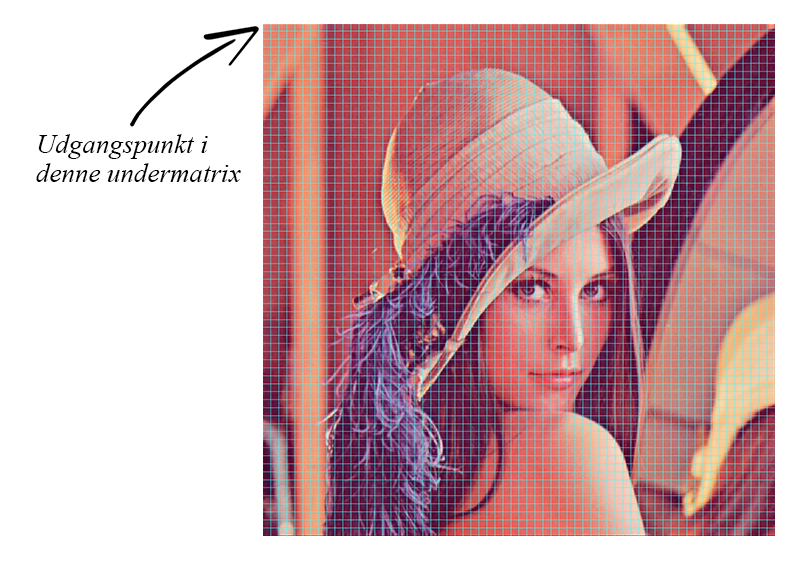
\includegraphics[width=0.5\textwidth]{billeder/lena-grid.png}
\caption{Lena delt op i 4096, $8 \times 8$ undermatricer.}
\label{fig:lena-grid-8x8}
\end{figure}
Herfra udføres DCT på undermatricen, og B findes vha. $B = U \boldsymbol{\cdot} A \boldsymbol{\cdot} U^T$, hvor $U$ og $U^T$ er givet i udtryk \vref{eq:DCTmatrix}.
\begin{figure}[!h]
\begin{minipage}[b]{0.25\linewidth}
\centering

\includegraphics[width=0.9\textwidth]{Billeder/LenaAnvendelse/RED8x8/lena2-R8x8-DCT.png}
\caption{DCT - Visuel.}
\label{fig:lena2-R8x8-DCT-visuel}
\end{minipage}
\hspace{0.5cm}
\begin{minipage}[b]{0.40\linewidth}
\centering
\[B_{1,\ 1}=\begin{bmatrix}
791    & -71  & 8,12   & 4,23   & -1,8  & -3,6  & -1,2  & 2,49   \\
-1,5  & 0,43  & 0,01   & 1,90   & 0,78  & 1,25   & -3,4  & -0,9 \\
-0,7 & -0,8 & -0,7 & -0,9 & -0,1 & -0,2 & 0,93  & 1,02   \\
2,66   & 1,02   & 1,38   & 0,21  & -0,5 & -0,5 & 0,95  & -1,3  \\
-3,3  & -0,9 & -1,5  & -0,2 & 0,75  & 0,18  & -1,0  & 1,55   \\
2,40   & 0,53  & 1,12   & 0,85  & -0,6 & 0,75  & -0,4 & -1,7  \\
-1,1  & -0,1 & -0,6 & -1,3  & 0,32  & -1,4  & 1,75   & 1,50   \\
0,21  & -0,1 & 0,18  & 0,98  & -0,1 & 1,15   & -1,6  & -0,9 \\
\end{bmatrix}\]
\caption{DCT - Tal.}
\label{fig:lena2-R8x8-DCT-matrix}
\end{minipage}
\end{figure}
Det ses tydeligt på den visuelle figur \ref{fig:lena2-R8x8-DCT-visuel}, hvordan alle overflødige høje frekvenser allerede er reduceret kraftigt. Dette er nøjagtigt det, som ønskes af DCT'en, da de lave frekvenser kan ses tydeligere af øjet end de høje. Den visuelle repræsentation er fremkommet ved at trunkere dataene til intervallet $[0;255]$. Næste trin i algoritmen er kvantiseringen, hvor der i dette eksempel tages udgangspunkt i $Q50$ jævnfør \vref{eq:Q50teori}. Den afrundede $C$ findes vha. \vref{C_beregning}
\begin{figure}[!h]
\begin{minipage}[b]{0.25\linewidth}
\centering

\includegraphics[width=0.9\textwidth]{Billeder/LenaAnvendelse/RED8x8/lena3-R8x8-quantization.png}
\caption{Kvantisering - Visuel.}
\label{fig:lena3-R8x8-quantization-visuel}
\end{minipage}
\hspace{0.5cm}
\begin{minipage}[b]{0.40\linewidth}
\centering
\[C_{1,\ 1}=\begin{bmatrix}
49 & -1 & 1 & . & . & . & . & . \\
.  & .  & . & . & . & . & . & . \\
.  & .  & . & . & . & . & . & . \\
.  & .  & . & . & . & . & . & . \\
.  & .  & . & . & . & . & . & . \\
.  & .  & . & . & . & . & . & . \\
.  & .  & . & . & . & . & . & . \\
.  & .  & . & . & . & . & . & . \\
\end{bmatrix}\]
\caption{Kvantisering - Tal.}
\label{fig:lena3-R8x8-quantization-matrix}
\end{minipage}
\end{figure}
Bemærk at der bruges indgangsvis division. Det ses, jævnfør tallene på figur \ref{fig:lena3-R8x8-quantization-matrix}, at matricen hovedsageligt udgøres af nuller. Dette er essentielt for Huffmankodningen, da den nu effektivt kan komprimere. Huffmantræet for undermatricen kan ses på figur \ref{fig:Huffman-8x8-visuel}. Tallene uden parentes repræsenterer hyppigheden af tallene i parentes.
\begin{figure}[htbp]
\centering
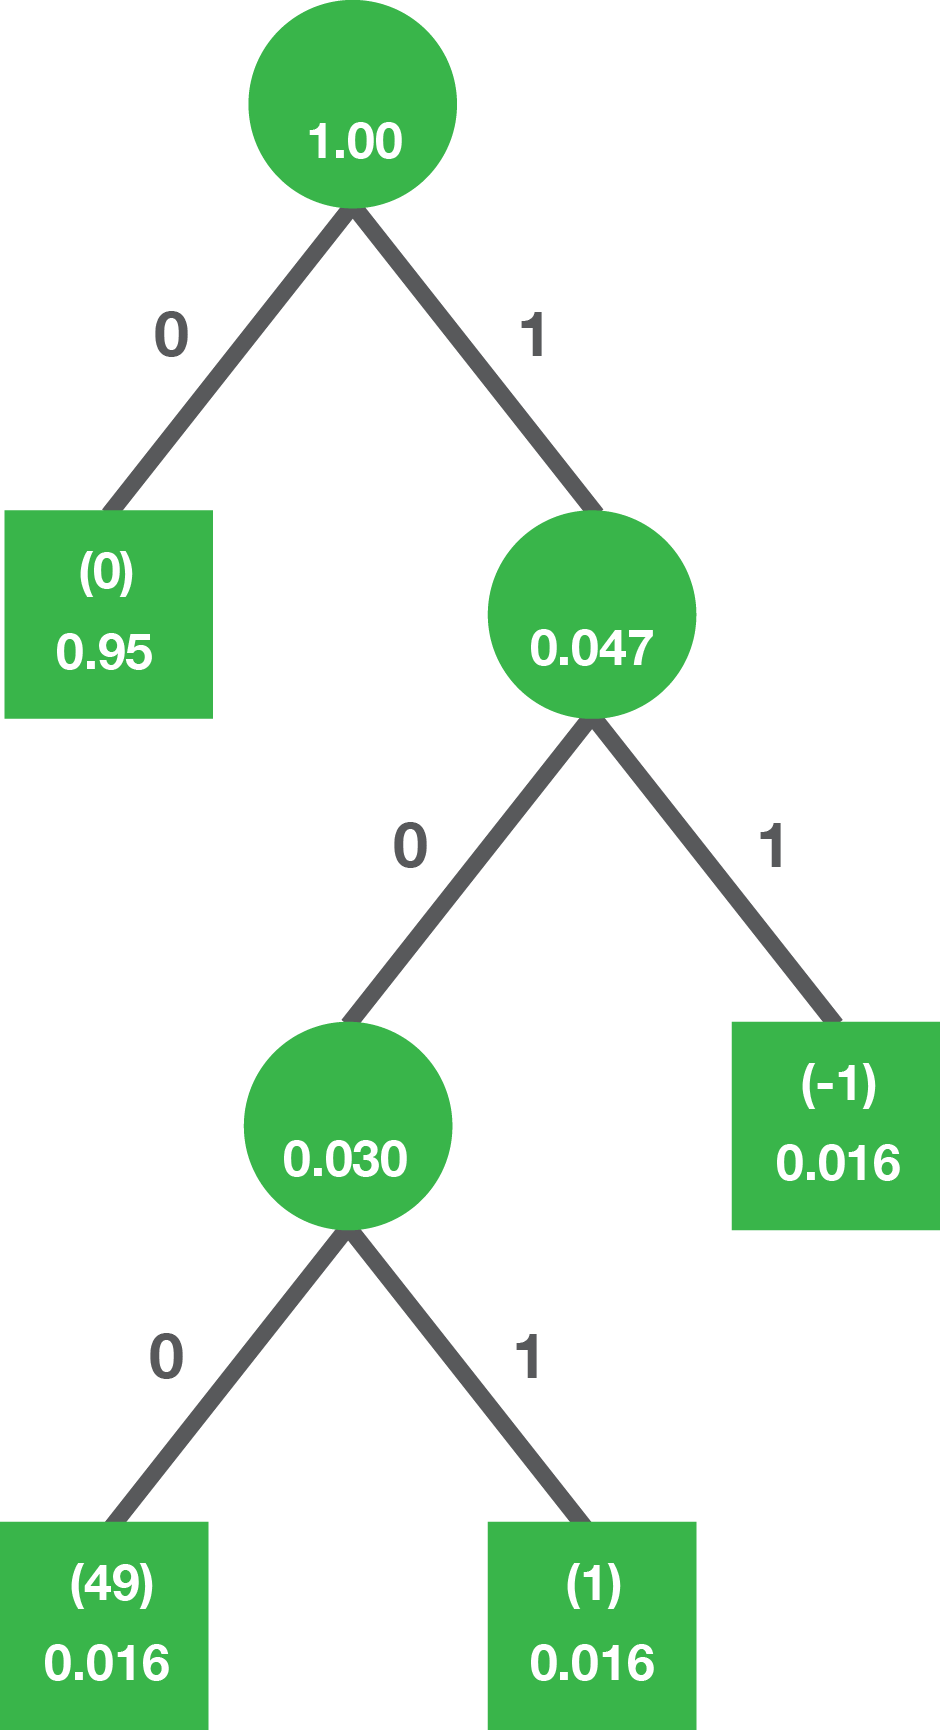
\includegraphics[width=0.25\textwidth]{Billeder/LenaAnvendelse/HUFFMAN/Huffman-8x8.png}
\caption{Huffmantræ for undermatricen.}
\label{fig:Huffman-8x8-visuel}
\end{figure}

Træet havde mildt sagt været markant større, hvis at Huffmantræet var lavet ud fra eksempelvis
 $A_{1,\ 1}$ eller $B_{1,\ 1}$. Her er det åbenlyst hvordan de to nævnte matricer, kun er \textit{forberedende} for en effektiv komprimering.

Der kan med fordel opstilles en tabel med relevante observationer fra Huffmantræet og dens resultater, se tabel \ref{tb:Huffman-8x8}. Den binære form blev fundet jævnfør \vref{sec:huffmanteori}.
\begin{table}[!h]
\centering
\begin{tabular}{|l|l|l|l|}
\hline
\textbf{Indgangsværdi} & \textbf{Antal} & \textbf{Sandsynlighed}      & \textbf{Binær form} \\ \hline
49                & 1              & $\frac{1}{64} \approx 0,016$ & 100                 \\ \hline
1                 & 1              & $\frac{1}{64} \approx 0,016$ & 101                 \\ \hline
-1                & 1              & $\frac{1}{64} \approx 0,016$ & 11                  \\ \hline
0                 & 61             & $\frac{61}{64} \approx 0,95$ & 0                   \\ \hline
\end{tabular}
\caption{Huffmantræet i tabelform}
\label{tb:Huffman-8x8}
\end{table}
I binær form vil undermatricen nu hedde: $$ 100110001010000000000000000000000000000000000000000000000000000000000 $$
En komprimeret fil er opnået, og den lange streng af nuller resulterer i, at filen fylder mindre, end hvis Huffmankodningen var blevet gjort før kvantiseringen. Jævnfør algoritmen på side \pageref{tb:Algoritme-Dekomprimering-DCT} udføres \textit{de}komprimeringen, hvilket gøres med de modsatte regneoperationer i forhold til komprimeringen.
\begin{table}[!h]
\centering
\begin{tabular}{lll}
\hline
\multicolumn{2}{l}{\textbf{Algoritme: Dekomprimering vha. DCT}}    &                                                                   \\ \hline
\\
\multicolumn{1}{|l}{1.}        & Input:                     & Komprimeret fil \\
\multicolumn{1}{|l}{2.}        & Output:                    & Dekomprimeret billede, $A'$                                           \\
                               &                            &                                                                   \\
\multicolumn{2}{|l}{\textit{Dekomprimering (invers proces)}} &                                                                   \\
\multicolumn{1}{|l}{9.}        & Entropidekodning:         & Filen dekomprimeres vha. Huffman til $C'$             \\
\multicolumn{1}{|l}{10.}        & Dekvantisering:            & $B' = Q_{(i,\ j)} \cdot C'_{(i,\ j)}$                                                 \\
\multicolumn{1}{|l}{11.}       & Invers DCT / DCT-III:      & $A' = U^T \boldsymbol{\cdot} B' \boldsymbol{\cdot} U$\\
\multicolumn{1}{|l}{12.}       & Decentrering omkring 0:      & $A' = A' + 128$ indgangsvist\\
\multicolumn{1}{|l}{13.}       & Samling:                   & $8 \times 8$ matricer samles til ét billede
\\  
\end{tabular}
\label{tb:Algoritme-Dekomprimering-DCT}
\end{table}
Resultatet af den inverse algoritme på $A_{(1,\ 1)}$ resulterer i værdierne illustreret i figur \ref{fig:lena4-R8x8-compressed-visuel} og \ref{fig:lena4-R8x8-decompressed-matrix}.
\begin{figure}[htbp]
\begin{minipage}[b]{0.27\linewidth}
\centering

\includegraphics[width=0.8\textwidth]{Billeder/LenaAnvendelse/RED8x8/lena4-R8x8-compressed.png}
\caption{Dekomprimeret - Visuel.}
\label{fig:lena4-R8x8-compressed-visuel}
\end{minipage}
\hspace{0.5cm}
\begin{minipage}[b]{0.45\linewidth}
\centering
\[\resizebox{0.9\textwidth}{!}{$C_{1,\ 1}=\begin{bmatrix}
226 & 225 & 224 & 224 & 225 & 226 & 228 & 230 \\
226 & 225 & 224 & 224 & 225 & 226 & 228 & 230 \\
226 & 225 & 224 & 224 & 225 & 226 & 228 & 230 \\
226 & 225 & 224 & 224 & 225 & 226 & 228 & 230 \\
226 & 225 & 224 & 224 & 225 & 226 & 228 & 230 \\
226 & 225 & 224 & 224 & 225 & 226 & 228 & 230 \\
226 & 225 & 224 & 224 & 225 & 226 & 228 & 230 \\
226 & 225 & 224 & 224 & 225 & 226 & 228 & 230 \\
\end{bmatrix}$}\]
\caption{Dekomprimeret - Tal.}
\label{fig:lena4-R8x8-decompressed-matrix}
\end{minipage}
\end{figure}
Den umiddelbare største ændring af undermatricen er dens endnu mere ensartethed. Da der ikke forekommer drastiske spring i overgangene mellem pixelene ser den monoton ud. Det er svært for det menneskelige øje, at skældne mellem denne undermatrice og den oprindelige, hvilket var intentionen i første omgang. 
For referencens skyld udføres algoritmen på hele Lena i de følgende figurer. Det undlades dog at vise den binære form.
%\begin{figure}[!h]
%\begin{minipage}{0.45\textwidth}
%\centering
%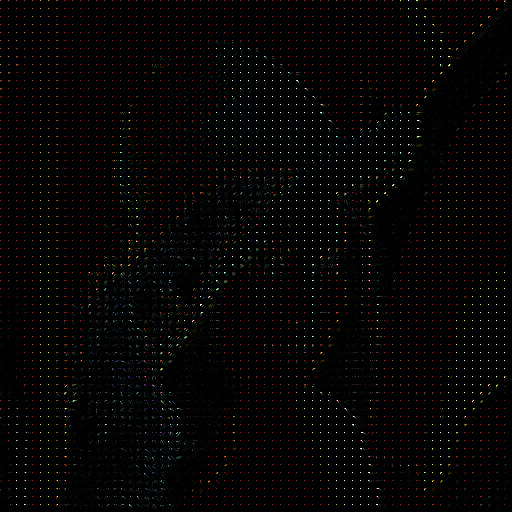
\includegraphics[width=0.4\textwidth]{Billeder/LenaAnvendelse/LENABILLEDE/lena2-DCT.png}
%\caption{DCT - Lena.}
%\label{fig:lena2-DCT-visuel}
%\end{minipage}
%\hspace{0.5cm}
%\begin{minipage}{0.45\textwidth}
%\centering
%
\includegraphics[width=0.4\textwidth]{Billeder/LenaAnvendelse/LENABILLEDE/lena4-enhanced-quantization2.png}
%\caption{Kvantisering - Lena.}
%\label{fig:lena4-enhanced-quantization-visuel}
%\end{minipage}
%\end{figure}
\begin{figure}[htbp]
\begin{minipage}{0.3\textwidth}
\centering
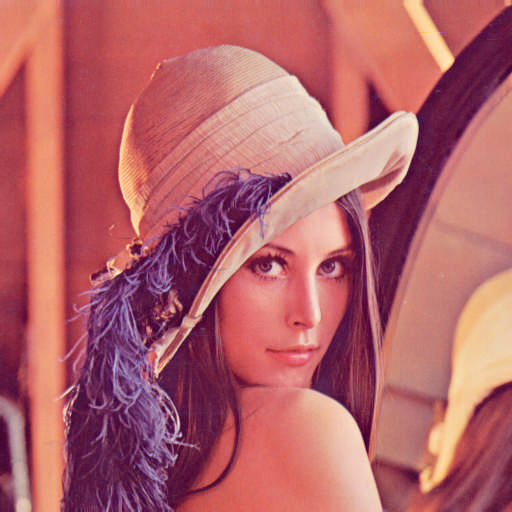
\includegraphics[width=0.9\textwidth]{Billeder/LenaAnvendelse/LENABILLEDE/lena5-compressed.png}
\caption{\href{https://www.dropbox.com/home/P1\%20-\%20B205/vejleder/billeder/DCT/Lena\%20ved\%20forskelige\%20Q?preview=lenaQ50.png}{Dekomprimeret - Lena.}}
\label{fig:lena5-decompressed-visuel}
\end{minipage}
\hspace{0.5cm}
\begin{minipage}{0.3\textwidth}
\centering

\includegraphics[width=0.9\textwidth]{Billeder/fejlbilleder/fejl50.png}
\caption{\href{https://www.dropbox.com/home/P1\%20-\%20B205/vejleder/billeder/DCT/Fejlbilleder?preview=fejl50.png}{Fejlbillede - Lena.}}
\label{fig:lena1-org-fejl}
\end{minipage}
\hspace{0.5cm}
\begin{minipage}{0.3\textwidth}
\centering
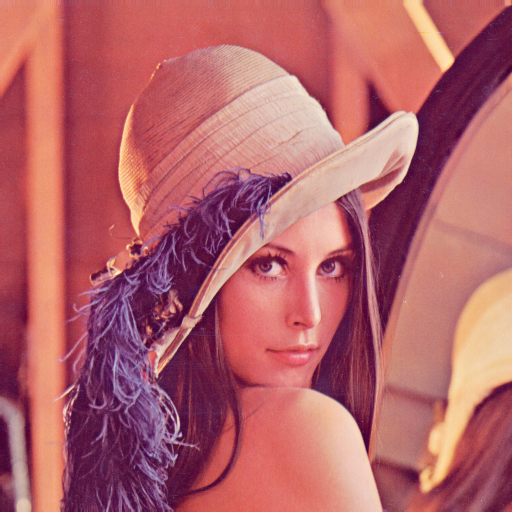
\includegraphics[width=0.9\textwidth]{Billeder/LenaAnvendelse/LENABILLEDE/lena1-org.png}
\caption{\href{https://www.dropbox.com/home/P1\%20-\%20B205/vejleder/billeder?preview=lena-org.tiff}{Oprindelig - Lena.}}
\label{fig:lena1-org-visuel}
\end{minipage}
\end{figure}
Jævnfør \ref{fig:lena5-decompressed-visuel} og \ref{fig:lena1-org-visuel} er det svært at skelne mellem billederne. Dette forstærkes ydermere af fejlbilledet, der illustrerer forskellen mellem det nye og det oprindelige billede. Grå illustrerer ingen forskel, sort illustrerer en mørkere farve i det nye billede, og ligeså illustrerer en lysere farve, at det nye billede er blevet lysere. En farvenuance illustrerer en farveforskel. Hensigten er opnået; billedet har ikke ændret sig betydeligt, og filstørrelsen er komprimeret i forhold til før algoritmen.